

%%%%%%%%%%%%%%%%%%%%%%%%%%%%%%%%%%%%%%%%%%%%%%%%%%%%%%%%%%%%%%%%%%%%%%%%%%%%%%%%%%%%%%%%%%%%%%%%%%%
\documentclass[10pt, a4paper]{article}
%%%%%%%%%%%%%%%%%%%%%%%%%%%%%%%%%%%%%%%%%%%%%%%%%%%%%%%%%%%%%%%%%%%%%%%%%%%%%%%%%%%%%%%%%%%%%%%%%%%

%--------------------------------------------------------------------------------------------------
% Dimensions :
%--------------------------------------------------------------------------------------------------

\setlength{\textheight}{26cm}
\setlength{\textwidth}{16cm}

\setlength{\topmargin}{-25mm}
\setlength{\oddsidemargin}{0mm}
\setlength{\evensidemargin}{0mm}

% \setlength{\columnsep}{20mm}

\setlength{\fboxsep}{1mm}
\setlength{\unitlength}{1mm}

%--------------------------------------------------------------------------------------------------
% Packages :
%--------------------------------------------------------------------------------------------------

\usepackage{latexsym}
\usepackage{graphicx}
\usepackage{pifont}
\usepackage{color}
\usepackage{amsmath}
\usepackage{amssymb}
\usepackage{enumerate}
 \usepackage{wasysym}

\usepackage[french]{babel}    % pour franciser le document

%\usepackage[latin1]{inputenc} % pour utiliser les caracteres accentues du claviers
\usepackage[utf8]{inputenc} 

\usepackage{accents}

\usepackage{cancel}
% Style des vecteurs : fleche ou gras ?

%\newcommand{\myvec}[1]{\boldsymbol{#1}}
\newcommand{\myvec}[1]{\vec{#1}}

\newcommand{\mytensor}[1]{\accentset{\Rightarrow}{#1}} % needs \usepackage{accents}

%---------------------------
% Operateurs differentiels :
%---------------------------

\newcommand{\divergence}{\mbox{\rm div}\,}

\newcommand{\gradient}{\myvec{\mbox{\rm gra}}\mbox{\rm d}}
% \newcommand{\gradient}{\mathbf{grad}\,}
% \newcommand{\ggradient}{\stackrel{\Rightarrow}{\mbox{gra}}\!\!\!\,\mbox{d}\,}
\newcommand{\ggradient}{\accentset{\Rightarrow}{\mbox{\rm gra}}\mbox{\rm d}\!}

%\renewcommand{\dot}[1]{\accentset{\hbox{\huge .}}{#1}}
\newcommand{\mydot}[1]{\accentset{\centerdot}{#1}}

\newcommand{\rot}{\vec{\mbox{\rm ro}}\mbox{\rm t}\,}
%\newcommand{\rot}{\mathbf{rot}\,}

% \newcommand{\vnabla}{\vec{\nabla}}
\newcommand{\vnabla}{\boldsymbol{\nabla}}

% Fonctions speciales:

\newcommand{\besselj}[1]{\mbox{J}_{#1}}
\newcommand{\besselk}[1]{\mbox{K}_{#1}}
\newcommand{\bessely}[1]{\mbox{Y}_{#1}}
\newcommand{\besseli}[1]{\mbox{I}_{#1}}

% Vecteurs, tenseurs et torseurs:

\newcommand{\ex}{\mathbf{e}_{x}}
\newcommand{\ey}{\mathbf{e}_{y}}
\newcommand{\ez}{\mathbf{e}_{z}}

\newcommand{\er}{\mathbf{e}_{r}}
\newcommand{\erho}{\mathbf{e}_{\rho}}
\newcommand{\ephi}{\mathbf{e}_{\varphi}}
\newcommand{\etheta}{\mathbf{e}_{\theta}}

%\newcommand{\tensor}[1]{\stackrel{\Rightarrow}{#1}}
\newcommand{\tensor}[1]{\mbox{\sl \textbf{#1}}}
\newcommand{\torseur}[4]{
   \!\!\!\! \left . \begin{array}{c} \\ \\ _#1 \end{array} \!\!\!
   \right \{ \!\!\!
   \begin{array}{#4} #2 \\ \\ #3 \end{array}}

% Integrales multiples:

\newcommand{\odblint}[1]{\int\!\!\!\!\!\int_{#1} \hskip -7mm \bigcirc \;}
\newcommand{\dblint}{\int\!\!\!\!\!\int}
\newcommand{\tplint}{\int\!\!\!\!\!\int\!\!\!\!\!\int}

% Fractions:

\renewcommand{\dfrac}[2]{\displaystyle \frac{#1}{#2}}

% Derivees ordinaires et partielles:

\newcommand{\dpdt}[1]{\dfrac{\partial #1}{\partial t}}
\newcommand{\dpdx}[1]{\dfrac{\partial #1}{\partial x}}
\newcommand{\dpdy}[1]{\dfrac{\partial #1}{\partial y}}
\newcommand{\dpdz}[1]{\dfrac{\partial #1}{\partial z}}

\newcommand{\ddpdt}[1]{\dfrac{\partial^2 #1}{\partial t^2}}
\newcommand{\ddpdx}[1]{\dfrac{\partial^2 #1}{\partial x^2}}
\newcommand{\ddpdy}[1]{\dfrac{\partial^2 #1}{\partial y^2}}
\newcommand{\ddpdz}[1]{\dfrac{\partial^2 #1}{\partial z^2}}

\newcommand{\dpdr}[1]{\dfrac{\partial #1}{\partial r}}
\newcommand{\dpdrho}[1]{\dfrac{\partial #1}{\partial \rho}}
\newcommand{\dpdphi}[1]{\dfrac{\partial #1}{\partial \varphi}}
\newcommand{\dpdtheta}[1]{\dfrac{\partial #1}{\partial \theta}}

\newcommand{\ddpdr}[1]{\dfrac{\partial^2 #1}{\partial r^2}}
\newcommand{\ddpdrho}[1]{\dfrac{\partial^2 #1}{\partial \rho^2}}
\newcommand{\ddpdphi}[1]{\dfrac{\partial^2 #1}{\partial \varphi^2}}
\newcommand{\ddpdtheta}[1]{\dfrac{\partial ^2#1}{\partial \theta^2}}

\newcommand{\ddt}[1]{\dfrac{d #1}{dt}}
\newcommand{\ddx}[1]{\dfrac{d #1}{dx}}
\newcommand{\ddy}[1]{\dfrac{d #1}{dy}}
\newcommand{\ddz}[1]{\dfrac{d #1}{dz}}
\newcommand{\ddr}[1]{\dfrac{d #1}{dr}}

\newcommand{\ddtref}[2]{\dfrac{d #1}{dt}_{\! | #2 }}
\newcommand{\dpdtref}[3]{\dfrac{\partial #1}{\partial #2}_{\! | #3 }}

% Misc:

\newcommand{\mycaption}[1]{\caption{\sl #1}}

\newcommand{\ligne}[1]{\hrule height #1\linethickness \hfill}

\newcommand{\thickline}[2]{\linethickness{#1} \line(1, 0){#2}}

\newcommand{\myline}{\noindent\underline{\hspace{\textwidth}}}
\newcommand{\mysection}[1]{\vskip 0.5cm \section{#1}\vskip -1.4cm 
   \myline \vskip 0.4cm \myline \bigskip}

\newcommand{\etal}{\textit{et al.}}

\newcommand{\varray}[1]{\renewcommand{\arraystretch}{#1}}

\newcommand{\puissance}[1]{^{\mbox{\footnotesize #1}}}
\newcommand{\indice}[1]{_{\mbox{\footnotesize #1}}}

%---------------------------------------------------------------------
% New environments:
%---------------------------------------------------------------------

\newcounter{MyEnumCounter}
\newcounter{MySaveCounter}
\newenvironment{MyEnum}{%
  \begin{list}{\arabic{MyEnumCounter}.}{\usecounter{MyEnumCounter}%
  \setcounter{MyEnumCounter}{\value{MySaveCounter}}}
  }{%
  \setcounter{MySaveCounter}{\value{MyEnumCounter}}\end{list}%
}
\newcommand{\MyEnumReset}{\setcounter{MySaveCounter}{0}}

\newenvironment{deuxcols}{\begin{tabular}{lr} \hspace*{-9.7mm}}{\end{tabular}}

\newenvironment{dem}{\noindent %
   \begin{tabular}{||l} \textsl{D\'emonstration :} \\ % 
   \begin{minipage}{15.5cm} \footnotesize} %
   {\end{minipage}\end{tabular}}

\newenvironment{abst}{\begin{quotation}\sl}{\end{quotation}}

\newenvironment{eqnbox}{\begin{equation}\begin{array}{|c|}  \hline \\ 
   \displaystyle}{\\ \\ \hline \end{array} \end{equation}}

\newcommand{\myprime}{\ \!'}

% JFM symbols:

\DeclareMathSymbol{\varGamma}{\mathord}{letters}{"00}
\DeclareMathSymbol{\varDelta}{\mathord}{letters}{"01}
\DeclareMathSymbol{\varTheta}{\mathord}{letters}{"02}
\DeclareMathSymbol{\varLambda}{\mathord}{letters}{"03}
\DeclareMathSymbol{\varXi}{\mathord}{letters}{"04}
\DeclareMathSymbol{\varPi}{\mathord}{letters}{"05}
\DeclareMathSymbol{\varSigma}{\mathord}{letters}{"06}
\DeclareMathSymbol{\varUpsilon}{\mathord}{letters}{"07}
\DeclareMathSymbol{\varPhi}{\mathord}{letters}{"08}
\DeclareMathSymbol{\varPsi}{\mathord}{letters}{"09}
\DeclareMathSymbol{\varOmega}{\mathord}{letters}{"0A}

% ---------------------------------------------------------------------
% MISC SYMBOLS :
% ---------------------------------------------------------------------

\font\SY=msam10 
\def\carreblanc{\hbox{\SY \char'3}}
\def\carrenoir{\hbox{\SY \char'4}}
\def\diamblanc{\hbox{\SY \char'6}}
\def\diamnoir{\hbox{\SY \char'7}}
\def\triblancright{\hbox{\SY \char'102}}
\def\triblancleft{\hbox{\SY \char'103}}
\def\triblancup{\hbox{\SY \char'115}}
\def\triblancdown{\hbox{\SY \char'117}}
\def\trinoirright{\hbox{\SY \char'111}}
\def\trinoirleft{\hbox{\SY \char'112}}
\def\trinoirup{\hbox{\SY \char'116}}
\def\trinoirdown{\hbox{\SY \char'110}}
\def\rondblanc{\hbox{\scriptsize $\bigcirc$}}
\def\rondnoir{\hbox{\LARGE $\bullet$}}

\font\BB=msbm10 scaled 1095
\def\setr{\hbox{\BB R}}
\def\setc{\hbox{\BB C}}
\def\setn{\hbox{\BB N}}
\def\setz{\hbox{\BB Z}}

% Pour enlever la numerotation des pages de la table des matieres:

%%%% debut macro, a placer dans preambule %%%%
\makeatletter
\def\addcontentsline@toc#1#2#3{%
   \addtocontents{#1}{\protect\thispagestyle{empty}}%
   \addtocontents{#1}{\protect\contentsline{#2}{#3}{\thepage}}}
\def\addcontentsline#1#2#3{%
  \expandafter\@ifundefined{addcontentsline@#1}%
  {\addtocontents{#1}{\protect\contentsline{#2}{#3}{\thepage}}}
  {\csname addcontentsline@#1\endcsname{#1}{#2}{#3}}}
\makeatother
%%%% fin macro %%%%

\newcommand{\titre}[1]{ %
  \medskip \noindent \underline{\makebox[\textwidth][l]{\textbf{#1}\textcolor{white}{pl}}}}% \\}

\newcommand{\sstitre}[1]{ %
  \bigskip \centerline{\textbf{#1}} \smallskip}

\def\draft{\overfullrule 5pt} % The \draft command marks the overful boxes

\def\indentlist{\list%
        {}{\labelwidth 0pt \leftmargin 3\labelsep}}
\let\endindentlist\endlist \relax

\def\datelist{\list%
        {}{\settowidth\labelwidth{[2001/02 :]}
        \leftmargin\labelwidth
        \advance\leftmargin\labelsep}
}
\let\enddatelist\endlist \relax

\def\longuelist{\list%
        {}{\settowidth\labelwidth{[Etablissement :]}
        \leftmargin\labelwidth
        \advance\leftmargin\labelsep}
}
\let\endlonguelist\endlist \relax

\def\shortlist{\list%
        {}{\settowidth\labelwidth{$\bullet$}
        \leftmargin\labelwidth
        \advance\leftmargin\labelsep}
}
\let\endshortlist\endlist \relax



%--------------------------------------------------------------------------------------------------
% Divers :
%--------------------------------------------------------------------------------------------------

\definecolor{rougefonce}{rgb}{0.7, 0.2, 0.2}

\renewcommand{\thickline}[2]{\linethickness{#1} \line(1, 0){#2}}
\renewcommand{\mycaption}[1]{\caption{\sl #1}}
\renewcommand{\myvec}[1]{\vec{#1}}

\newcommand{\footnoteremember}[2]{
\footnote{#2}
\newcounter{#1}
\setcounter{#1}{\value{footnote}}% \!\!\!
}
\newcommand{\footnoterecall}[1]{
\footnotemark[\value{#1}]
}

% \pagestyle{empty}

\graphicspath{{Figures/}} % chemin d'acces au repertoire des figures (par ex.)

%%%%%%%%%%%%%%%%%%%%%%%%%%%%%%%%%%%%%%%%%%%%%%%%%%%%%%%%%%%%%%%%%%%%%%%%%%%%%%%%%%%%%%%%%%%%%%%%%%%
\begin{document}
%%%%%%%%%%%%%%%%%%%%%%%%%%%%%%%%%%%%%%%%%%%%%%%%%%%%%%%%%%%%%%%%%%%%%%%%%%%%%%%%%%%%%%%%%%%%%%%%%%%

\begin{center}

  \textsc{Université Toulouse 3 -- Paul Sabatier \hfill Année universitaire 2015-2016}
  
  \textsc{Mécanique des fluides \hfill L3 Mécanique}
  
  \vspace{0mm}
  
  \begin{center}
    \thickline{0.4mm}{160}
    \\ \vspace{3mm}
  \textbf{\large Exercice complémentaire 7.0 : Estimation de la traînée d'un cylindre}
    \\ %\vspace{1mm}
    \thickline{0.4mm}{160}
  \end{center}

%  \vspace{0mm}
  
\end{center}

%\stepcounter{section}

\medskip

\begin{enumerate}
\item Notons $\Omega$ le {\em volume de contrôle } correspondant au parallélépipède dont on a retiré le cylindre.
Notons $\partial \Omega = \Gamma \cup \Sigma$ la frontière du volume de contrôle, où $\Sigma$ est la surface du cylindre et 
$\Gamma$ la frontière "fluide" du domaine (les faces extérieures).


Le bilan de masse $M(\Omega) = \iiint_{\Omega} \rho dV$ sur $\Omega$ s'écrit :
$$
\frac{ d }{ d t} M(\Omega) = - \oiint_{\partial \Omega} \rho \vec u \cdot \vec n \,d S   = 0.
$$
En notant que l'intégrale sur $\Sigma$ est nulle (car $\vec u \cdot \vec n = 0$ sur $\Sigma$), on arrive à 
$$ - \oiint_{\Gamma} \rho \vec u \cdot \vec n \,d S = 0.
$$

Evaluons l'intégrale sur chacune des 6 faces extérieures du domaine. Les 4 premières faces correspondent aux cotés du rectangle représenté sur la figure multipliés par la profondeur ($ 2H$). Les 2 dernières faces (en $z = \pm H$) ne contribuent pas au bilan car il n'y a pas de vitesse dans la direction $z$. Donc : 
\begin{eqnarray*}
0  = &- \rho  &  \left[  \int_{-H}^H \int_{-b}^b  \vec u(-L,y) \cdot \vec n \, d y \, dz  + \int_{-H}^H \int_{-b}^b \vec u(+L,y) \cdot \vec n \, d y \, dz  \right.
\\
&+&\left.  \int_{-H}^H \int_{-L}^L \vec u (x,-b) \cdot \vec n \, dx  \, dz+ \int_{-H}^H \int_{-L}^L  \vec u (x,b) \cdot \vec n \, dx \, dz   \right]
\end{eqnarray*} 

En remplaçant la normale $\vec  n$ par sa valeur sur chacune des faces (respectivement $-\vec e_x, + \vec e_x, -\vec e_y$ et $+\vec e_y$) , on arrive à :
\begin{equation} 
2 H  \rho  \left[ 2 b U_0  - \int_{-b}^b u(+L,y) \, d y + \int_{-L}^L v(x,-b) \, dx - \int_{-L}^L v(x,b) \, dx  \right] = 0
 \label{eq:masse}
\end{equation}

\item 
Ecrivons de même le bilan intégral pour la quantité de mouvement totale $\vec P(\Omega) = \iiint \rho \vec u \, dV$ contenue dans le volume de contrôle :

$$
\frac{ d }{ d t} \vec{P}(\Omega) = \oiint_{\partial \Omega} (  - p \vec{n}  + \mytensor{\tau} \cdot \vec n ) \, dS -  \oiint_{\partial \Omega}  (\rho \vec u)  (\vec u \cdot \vec n) \,d S  
$$

Dans le cas stationnaire ($\frac{ d }{ d t} \vec{P}(\Omega) = 0$)
\footnote{ En toute rigueur, l'écoulement étant fortement instationnaire, la quantité de mouvement $P(\Omega)$ varie au cours du temps ; cependant le raisonnement reste valable si $\vec F_{{\cal F} -> \Sigma}$ est la force {\em moyenne} exercée sur le cylindre} ,
Et en séparant les contributions sur $\Sigma$ et sur $\Gamma$, on arrive au théorème d'Euler : 
$$
\vec F_{{\cal F} -> \Sigma} = - \oiint [ p \vec n + ( \rho \vec u) (\vec u \cdot \vec n ) ]  dS
$$    
Evaluons comme dans la question précécente les intégrales  sur chacune des 4 faces. En notant que les contributions de pression s'annulent on a: 
\begin{eqnarray*}
\vec F_{{\cal F} -> \Sigma} &=& 
- \left[  \int_{-H}^H \int_{-b}^b  \rho ( U_0 \vec e_x)  (- U_0 ) \, d y \, dz  + \int_{-H}^H \int_{-b}^b  \rho ( u(L,y) \vec e_x) (+ u(L,y))  \, d y \, dz  \right.
\\
&+&\left.  \int_{-H}^H \int_{-L}^L \rho (U_0 \vec e_x +v(x,-H) \vec e_y ) (- v(x,-H)) \, dx  \, dz+ \int_{-H}^H \int_{-L}^L  \rho (U_0 \vec e_x +v(x,+H) \vec e_y ) (+ v(x,H)) \, dx \, dz   \right]
\end{eqnarray*}

 La composante selon $\vec e_x$ (traînée) s'obtient en projetant l'équation précédente le long de cette direction.
On arrive finalement à :
 
\begin{equation}
F_x = \vec F_{{\cal F} -> \Sigma}  \cdot \vec  e_x 
= 2 H \rho   \left[ 2 b U_0^2   - \int_{-b}^b (u(+L,y))^2  \, d y + \int_{-L}^L U_0 v(x,-b) \, dx - \int_{-L}^{L} U_0 v(x,b) \, dx  \right]
 \end{equation}

\item
Combinons maintenant les deux équations (1) et (2) en faisant la combinaison (2) - $U_0$ (1). On remarque que tous les termes se simplifient à l'exception de l'intégrale dans le plan de sortie  et qu'on arrive à :

\begin{equation}
F_x 
= 2 H \rho  \int_{-b}^b u(+L,y) ( U_0- u(+L,y) )  \, d y   
 \end{equation}
L'interprétation physique de cette équation est : {\em la force de traînée est égale au flux du déficit de vitesse à travers le plan de sortie.}


\item Avec le profil de vitesse indiqué on arrive à :

$$
F_x 
= 2 H \rho \left[ \int_{-b}^{-a}  U_0 ( U_0- U_0 )  \, d y +\int_{-a}^{a}  0.7 U_0 ( U_0- 0.7 U_0 )\, dy  +\int_{a}^{b}  U_0 ( U_0- U_0 ) \, dy \right]
= (2 H) \cdot ( 2 a) \cdot 0.21 \rho U_0^3  
$$

Le coefficient de traînée correspondant est 
$$
C_x = \frac{F_x}{(1/2) \rho S U_0^2} = 0.42
$$

où $S = (2 H) \cdot (2a) $ est la surface frontale du cylindre.

\item
En projetant le bilan de QDM selon $\vec e_y$, on obtient :

\begin{equation}
F_y = \vec F_{{\cal F} -> \Sigma}  \cdot \vec  e_y 
= 2 H \rho   \left[ \int_{-L}^L v(x,-b)^2 \, dx - \int_{-L}^{L} v(x,b)^2 \, dx  \right]
 \end{equation}

On remarque que si $|v(x,+b)| = |v(x,-b)|$, la portance est nulle.



\end{enumerate}


\end{document}

%==================================================================================================
\section{Recherche d'une solution particulière}
%==================================================================================================


\begin{myenumerate}
\item 
\begin{enumerate}[a)]
\item 
  La conduite est immobile et les pressions d'entrée et de sortie sont fixées 
  et ne varient donc pas au cours du temps.
  Aucune condition limite et aucun paramètre du problème ne dépendant du temps
  (on parle alors d'\textsl{invariance temporelle}),
  il est donc légitime de chercher une solution de même nature :
  \dotfill \fbox{$\myvec{u} = \myvec{u}(r, \theta, z)$}
\item 
	La conduite est de très grande longueur par rapport au rayon ($R/L \ll 1$).
	On peut donc modéliser le problème par une conduite supposée géométriquement
	\textsl{infinie} dans la direction $z$ et donc \textsl{invariante}
	dans cette direction.
  Aucune condition limite et aucun paramètre du problème ne dépendant de $z$
  (on parle alors d'\textsl{invariance suivant $z$}),
  il est donc légitime de chercher une solution de même nature :
  \dotfill \fbox{$\myvec{u} = \myvec{u}(r, \theta)$}
\item
	La conduite est supposée parfaitement cylindrique, 
	donc de symétrie de rotation (ou \textsl{axisymétrique}) 
	autour de l'axe $Oz$.
  Aucune condition limite et aucun paramètre du problème ne dépendant de $\theta$
  (on parle alors d'\textsl{invariance par rotation autour de l'axe $Oz$}),
  il est donc légitime de chercher une solution de même nature :
  \dotfill \fbox{$\myvec{u} = \myvec{u}(r)$}
\item 
	Le fluide est mis en mouvement par la différence de pression entre l'entrée et la sortie
	de la conduite. La force associé à ce gradient de pression est dirigée suivant $z$,
	et il n'existe pas de force extérieure dans les autres directions.
	Dans ces conditions, il est naturel de chercher une solution d'écoulement aligné
	avec cette force motrice suivant $z$ 
  \dotfill \fbox{$\myvec{u} = u(r) \, \ez$}
\end{enumerate}
\item
En repérage cylindrique (cf. fascicule de TD) :
$\divergence \myvec{u}
= \dfrac{1}{r} \dpdr{}\left (r u_r \right) + \dfrac{1}{r} \dpdtheta{u_{\theta}} + \dpdz{u_z}$

Comme $u_r = u_\theta = 0$ et $u_z = u(r)$, on vérifie bien que
\dotfill
\fbox{$\divergence \myvec{u} = 0$}

\medskip
\item
	Le tenseur des contraintes $\mytensor{\sigma}$ 
	a pour expression (cf. annexe du fascicule de TD) :
	\begin{eqnarray*}
		\mytensor{\sigma}
		 & = & 
		\left (
		\begin{array}{ccc}
			\sigma_{rr} & \sigma_{r\theta} & \sigma_{rz} \\
			\sigma_{r\theta} & \sigma_{\theta\theta} & \sigma_{\theta z} \\
			\sigma_{rz} & \sigma_{\theta z} & \sigma_{zz}
		\end{array}
		\right )
		=
		\left (
		\begin{array}{ccc}
			- p + \tau_{rr} & \tau_{r\theta} & \tau_{rz} \\
			\tau_{r\theta} & -p + \tau_{\theta\theta} & \tau_{\theta z} \\
			\tau_{rz} & \tau_{\theta z} & -p + \tau_{zz}
		\end{array}
		\right )	
		\\	 & & \\ & & \\
		& = &
		\left (
		\begin{array}{ccccc}
			- p + 2\mu \dpdr{u_r} 
			& & 
			\mu \left( \dfrac{1}{r} \dpdtheta{u_r} + \dpdr{u_{\theta}} - \dfrac{u_{\theta}}{r} \right) 
			& & 
			\mu \left ( \dpdr{u_z} + \dpdz{u_r} \right ) 
			\\ & & & & \\
			\mu \left( \dfrac{1}{r} \dpdtheta{u_r} + \dpdr{u_{\theta}} - \dfrac{u_{\theta}}{r} \right) 
			& & 
			-p + 2\mu \left( \dfrac{1}{r}\dpdtheta{u_\theta} + \dfrac{u_r}{r} \right) 
			& & 
			\mu \left( \dpdz{u_\theta} + \dfrac{1}{r} \dpdtheta{u_z} \right) 
			\\ & & & & \\
			\mu \left ( \dpdr{u_z} + \dpdz{u_r} \right ) 
			& & 
			\mu \left( \dpdz{u_\theta} + \dfrac{1}{r} \dpdtheta{u_z} \right)
			& & 
			-p + 2\mu \dpdz{u_z}
		\end{array}
		\right )		
	\end{eqnarray*}
	soit, 
	pour cette solution d'écoulement particulière
	avec $u_r = u_\theta = 0$ et $u_z = u(r)$ :
	
	\medskip
	\dotfill
	\fbox{$
		\mytensor{\sigma}
		 =
		\left (
		\begin{array}{ccc}
			-p & 0 & \mu \dpdr{u} \\ & & \\
			0 & -p & 0 \\ & & \\
			\mu \dpdr{u} & 0 & -p
		\end{array}
		\right )
	$}
\end{myenumerate}

%==================================================================================================
\section{Mise en équation}
%==================================================================================================

\begin{myenumerate}
\item
\begin{enumerate}[a)]
\item 
La composante radiale (suivant $\er$) de l'équation de Navier-Stokes s'écrit (cf. fascicule de TD) :

\medskip %\hspace{-5mm}
$
\dpdt{u_r}
+ 
u_r \dpdr{u_r} + \dfrac{u_{\theta}}{r} \dpdtheta{u_r} + u_z \dpdz{u_r} - \dfrac{u_{\theta}^2}{r} 
=
- \dfrac{1}{\rho} \dpdr{p}
+ \nu \left[ \dfrac{1}{r} \dpdr{} \left( r \dpdr{u_r} \right) + 
             \dfrac{1}{r^2} \ddpdtheta{u_r} + \ddpdz{u_r} -
             \dfrac{u_r}{r^2} - \dfrac{2}{r^2} \dpdtheta{u_{\theta}} \right]
$

\medskip
Comme $u_r = u_\theta = 0$, il reste $0 = - \dfrac{1}{\rho} \dpdr{p}$ soit $\dpdr{p} = 0$ donc
\dotfill
\fbox{$p$ ne dépend pas de $r$}

\medskip
La composante azimutale (suivant $\myvec{e}_\theta$) de l'équation de Navier-Stokes s'écrit :

\medskip %\hspace{-5mm}
$
\dpdt{u_\theta}
+ 
u_r \dpdr{u_\theta} + \dfrac{u_{\theta}}{r} \dpdtheta{u_\theta} + u_z \dpdz{u_\theta} + \dfrac{u_ru_{\theta}}{r} 
=
- \dfrac{1}{\rho r} \dpdtheta{p}
+ \nu \left[ \dfrac{1}{r} \dpdr{} \left( r \dpdr{u_\theta} \right) + 
             \dfrac{1}{r^2} \ddpdtheta{u_\theta} + \ddpdz{u_\theta} -
             \dfrac{u_\theta}{r^2} + \dfrac{2}{r^2} \dpdtheta{u_r} \right]
$

\medskip
Comme $u_r = u_\theta = 0$, il reste $0 = - \dfrac{1}{\rho r} \dpdtheta{p}$ soit $\dpdtheta{p} = 0$ donc
\dotfill
\fbox{$p$ ne dépend pas de $\theta$}

\item
D'après la question précédente $p=p(z)$ uniquement.

La composante axiale (suivant $\ez$) de l'équation de Navier-Stokes s'écrit :

\medskip
$
\dpdt{u_z} + u_r \dpdr{u_z} + \dfrac{u_{\theta}}{r} \dpdtheta{u_z} + u_z \dpdz{u_z} =
- \dfrac{1}{\rho} \ddz{p}
+ \nu \left[ \frac{1}{r} \dpdr{} \left( r \dpdr{u_z} \right) + 
             \dfrac{1}{r^2} \ddpdtheta{u_z} + \ddpdz{u_z} \right]
$

\medskip
Comme $u_r = u_\theta = 0$ et $u_z = u(r)$, il reste
\dotfill 
$\ddz{p} = \mu \dfrac{1}{r} \dpdr{} \left ( r \dpdr{u} \right )$

Le terme de gauche est une fonction de $z$ uniquement et le terme de droite est une fonction de $r$ uniquement : 
par conséquent chacun de ces termes est nécessairement constant.

\medskip
En particulier \fbox{le gradient de pression est constant} : \qquad
$\ddz{p} = A \quad \Leftrightarrow \quad p(z) = Az+B$,

\medskip
où $A$ et $B$ sont des constantes à déterminer d'après les conditions limites.
Entre l'entrée et la sortie distantes de $L$, la pression passe de $P_1$ à $P_2$.
En notant $z_1$ et $z_2$ les positions de l'entrée et de la sortie, on a
$\Delta P = P_2 - P_1 = p(z_2) - p(z_1) = A (z_2-z_1) = AL$
d'où $A = (P_2-P_1)/L = -G$.

\medskip
On en déduit
\dotfill
\fbox{$\ddz{p} = -G = \dfrac{P_2-P_1}{L} = \dfrac{\Delta P}{L}$}

\medskip
\item
On a vu dans la question précédente que la composante axiale de l'équation de Navier-Stokes
s'écrivait dans le cas présent :

\medskip
$\ddz{p} = \mu \dfrac{1}{r} \dpdr{} \left ( r \dpdr{u} \right )$,
c'est-à-dire
\dotfill
\fbox{$\dpdr{} \left ( r \dpdr{u} \right ) = -\dfrac{Gr}{\mu}$}
\end{enumerate}

\medskip
\item
	Question subsidiaire :
\begin{enumerate}[a)]
\item 
	On cherche un écoulement de la forme $\myvec{u} = u(r) \, \ez$ : les trajectoires des
	particules fluides sont donc rectilignes, et leur accélération dans les directions radiale $r$
	et azimutale $\theta$ sont donc nulles. 
	On peut donc faire raisonnablement l'hypothèse a priori 
	que le gradient de pression dans ces directions est nul, et donc que la pression ne dépend
	ni de $r$ ni de $\theta$
	\dotfill
	\fbox{$p=p(z)$}
\item
	Le bilan de quantité de mouvement horizontale (\textsl{suivant $z$}) 
	$\rho u$ pour le volume de contrôle $\varOmega$
	de rayon $r$ et de longueur infinitésimale $dz$ s'écrit :
	\[
		\dpdt{} \int_\varOmega \rho u \, dV
		=
		\oint_{\partial \varOmega}
		\left (\mytensor{\sigma} \cdot \myvec{n} \right ) \cdot \ez \, dS
		- 
		\oint_{\partial \varOmega}
		\rho u \left ( \myvec{u} \cdot \myvec{n} \right ) \, dS
	\]
	Le terme de gauche est nul car l'écoulement est stationnaire.
	Le dernier terme de droite correspond au flux de quantité de mouvement horizontale : 
	comme l'écoulement est unidirectionnel et invariant suivant $z$, toute la quantité de mouvement 
	qui rentre à droite en $z$ ressort exactement à l'identique en $z+dz$.
	Le flux de quantité de mouvement horizontale est donc nul (je vous conseille de 
	retrouver ce résultat en détaillant 
	l'intégrale sur tous les éléments de frontière du volume de contrôle).
	
	Il reste donc le terme correspondant aux forces horizontales de contraintes exercées par l'exté\-rieur 
	sur le fluide à l'intérieur du volume de contrôle.
	Il s'agit des forces de pression sur les sections d'entrée et de sortie, et la force de frottement
	visqueux sur la surface cylindrique de rayon $r$ et de longueur $dz$.
	
	Le bilan s'écrit alors :
	$ 0 = p(z) \times \pi r^2 - p(z+dz) \times \pi r^2 + \tau(r) \times 2\pi r\, dz$
	(comme précédemment vous pouvez 
	retrouver ce résultat en détaillant 
	l'intégrale de la contrainte sur tous les éléments de frontière du volume de contrôle).
	Dans cette expression $\tau = \tau_{rz}$ est la contrainte suivant $z$ exercée sur la facette de normale $\er$.
	L'écoulement ne dépendant que de $r$, cette contrainte ne dépend que de~$r$.
	
	En divisant par $dz\rightarrow 0$, on en déduit l'équation : \qquad
	$\ddz{p}(z) = \dfrac{2}{r} \; \tau(r)$
	
	\medskip
	Le terme de gauche est une fonction de $z$ uniquement et le terme de droite est une fonction de $r$ uniquement : 
	par conséquent chacun de ces termes est nécessairement constant.
	
	\medskip
	Le raisonnement est alors identifique à celui de la question 4b, et on en déduit que $\ddz{p} = -G$
	
	\medskip
	et donc que 
	\dotfill
	\fbox{$\tau(r) = -\dfrac{Gr}{2}$}
	
\medskip
\item
	Dans l'hypothèse d'un fluide newtonien, on a : \quad $\tau = \tau_{rz} = \mu \dpdr{u_z} = \mu \dpdr{u}$
	
	D'où l'équation pour $u(r)$ : 
	\dotfill
	\fbox{$\dpdr{u} = -\dfrac{Gr}{2\mu}$}

\medskip
Remarque : cette équation s'intègre directement et donne la solution générale $u(r) = -\dfrac{Gr^2}{4\mu} + A$

\smallskip
où $A$ est une constante à définir avec la condition limite d'adhérence à la paroi $u(R) = 0$,

\smallskip
d'où $A = \dfrac{GR^2}{4\mu}$ et
\dotfill $u(r) = \dfrac{GR^2}{4\mu} \left [ 1 - \left (  \dfrac{r}{R} \right)^2 \right ]$

\medskip
Bien évidemment on retrouvera cette solution d'écoulement en résolvant l'équation (2) issue de la question 4c.
C'est l'objet de la section suivante.

\end{enumerate}
\end{myenumerate}


%==================================================================================================
\section{Résolution et applications}
%==================================================================================================

\begin{myenumerate}
\item
L'équation (2) à résoudre (cf. question 4c) s'écrit :

\medskip
$\dpdr{} \left ( r \dpdr{u} \right ) = -\dfrac{Gr}{\mu}
\; \Leftrightarrow \;
r \dpdr{u} = -\dfrac{Gr^2}{2\mu} + A
\; \Leftrightarrow \;
\dpdr{u} = -\dfrac{Gr}{2\mu} + \dfrac{A}{r}
\; \Leftrightarrow \;
u(r) = -\dfrac{Gr^2}{4\mu} + A\, \log(r) + B
$

\medskip
Les constantes d'intégration $A$ et $B$ sont à déterminer à l'aide des conditions limites.

\medskip
La vitesse doit être finie sur l'axe $r=0$ :
comme $\log (r\rightarrow 0) \rightarrow -\infty$, alors nécessairement $A=0$.

\medskip
Il y a adhérence à la paroi : \quad
$u(r=R) = 0 
\; \Leftrightarrow \;
0 = -\dfrac{GR^2}{4\mu} + B
\; \Leftrightarrow \;
B = \dfrac{GR^2}{4\mu}
$

\medskip
On en déduit \dotfill
\fbox{$ u(r) 
= \dfrac{G}{4\mu} \left ( R^2 - r^2\right ) 
= \dfrac{GR^2}{4\mu} \left [ 1 - \left (  \dfrac{r}{R} \right)^2 \right ]
= - \dfrac{R^2}{4\mu} \, \ddx{p} \left [ 1 - \left (  \dfrac{r}{R} \right)^2 \right ] $}

\medskip
L'écoulement solution, appelé \textsl{écoulement de Poiseuille},
correspond donc à un profil de vitesse parabolique
(remarque : il s'agit bien du même écoulement que celui trouvé dans la question 5c).
Le profil de vitesse est tracé sur la figure ci-dessous.

\vspace{5mm}
\begin{center}
\begin{picture}(80, 50)(0, 0)
	\put(0, 0){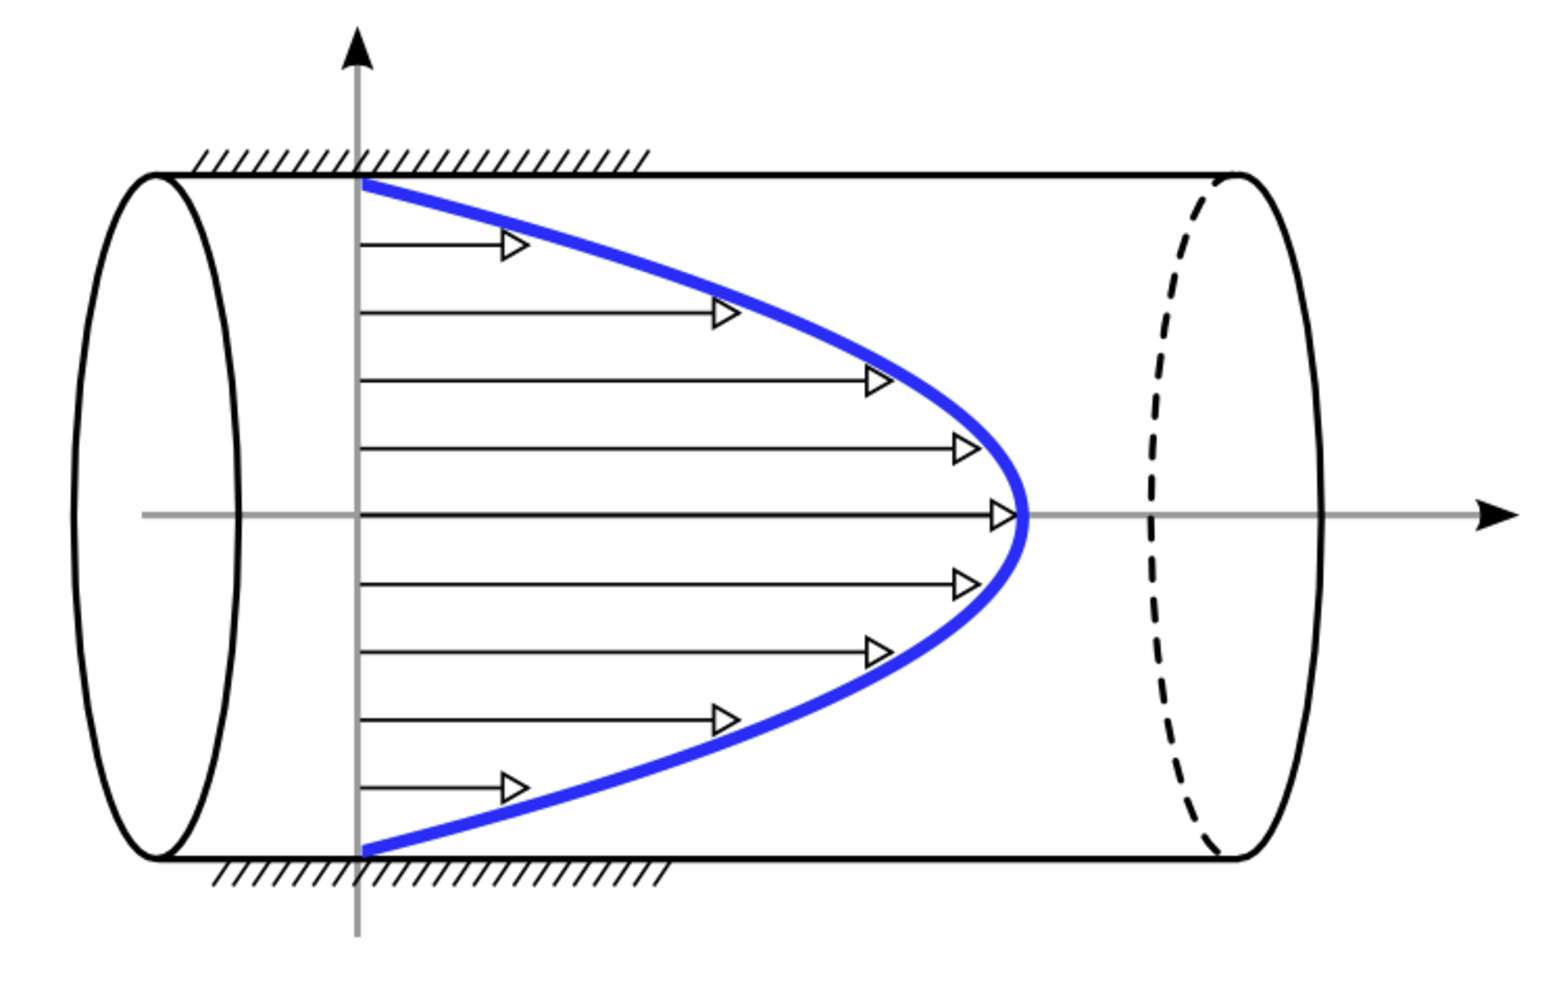
\includegraphics[width=80mm]{poiseuille.pdf}}
	\put(18, 51){$r$}
	\put(79, 23.5){$z$}
	\put(15, 38){$R$}
	\put(16, 25){$0$}
	\put(17.5, 23.5){\scriptsize $\bullet$}
	\put(50, 30){\color{blue}{$u(r)$}}
\end{picture}
\end{center}

\item
	Le débit massique passant à travers la section $S$ de la conduite
	est donné par 
	
	\medskip
	$\displaystyle \dot{m} = \int_S \rho \, \myvec{u} \cdot \myvec{n} \, dS = \int_0^R \rho \, u(r) \, 2\pi r\, dr
	= \dfrac{\pi \rho GR^2}{2\mu} \int_0^R \left ( r - \dfrac{r^3}{R^2} \right ) \, dr
	= \dfrac{\pi GR^2}{2\nu} \left [ \dfrac{R^2}{2} - \dfrac{R^2}{4} \right ]$ car $\mu = \rho \nu$
	
	\medskip
	soit \dotfill \fbox{$\dot{m} = \dfrac{\pi GR^4}{8\nu} = - \dfrac{\pi R^4}{8\nu} \ddx{p}$ }
	
	\medskip
	En remarquant que pour un fluide homogène $\rho = Cte$ :
	
	$\displaystyle \dot{m} = \int_S \rho \, \myvec{u} \cdot \myvec{n} \, dS 
	= \rho \int_S \, \myvec{u} \cdot \myvec{n} \, dS = \rho \, q$
	où $q$ correspond au débit volumique à travers la section $S$,
	
	on en déduit
	\dotfill
	\fbox{$q = \dfrac{\pi GR^4}{8\mu} = - \dfrac{\pi R^4}{8\mu} \ddx{p}$}
	
	\medskip
	La vitesse moyenne est donnée par $\displaystyle U = \dfrac{1}{S} \int_S \, \myvec{u} \cdot \myvec{n} \, dS 
	= \dfrac{q}{S}$
	
	où $S = \pi R^2$ désigne la surface de la section de la conduite, d'où
	\dotfill
	\fbox{$U = \dfrac{GR^2}{8\mu} = - \dfrac{R^2}{8\mu} \ddx{p}$}
	
	\medskip
	On remarque que la vitesse maximale se trouve sur l'axe $r=0$ : \hfill
	\fbox{$U\indice{max} = \dfrac{GR^2}{4\mu} = - \dfrac{R^2}{4\mu} \ddx{p} = 2 U$}
\end{myenumerate}\end{document}

\item
	Déterminer l'expression de la contrainte visqueuse $\tau(r)$ et discuter de son signe.
	Où l'intensité de cette contrainte est-elle maximale ? 
\item
	En déduire la force exercée par l'écoulement sur la conduite de longueur $L$.
\item
	Retrouver le résultat en écrivant un bilan global d'énergie cinétique dans la conduite.
\item
	Déterminer la dissipation d'énergie cinétique dans la conduite de longueur $L$.
\item
	La chute de pression dans la conduite correspond à une diminution de l'énergie mécanique 
	du fluide à cause des frottements visqueux. On parle alors de perte de charge régulière
	et on définit le coefficient de perte de charge par 
	\begin{equation}
		\lambda = \dfrac{D}{L} \times \dfrac{P_1-P_2}{\frac{1}{2} \rho U^2}
	\end{equation}	
	Vérifier que ce coefficient est sans dimension, et déterminer son expression en fonction
	du nombre de Reynolds dans le cas de l'écoulement de Poiseuille. 
\end{myenumerate}

%%%%%%%%%%%%%%%%%%%%%%%%%%%%%%%%%%%%%%%%%%%%%%%%%%%%%%%%%%%%%%%%%%%%%%%%%%%%%%%%%%%%%%%%%%%%%%%%%%%
\end{document}
%%%%%%%%%%%%%%%%%%%%%%%%%%%%%%%%%%%%%%%%%%%%%%%%%%%%%%%%%%%%%%%%%%%%%%%%%%%%%%%%%%%%%%%%%%%%%%%%%%%

